\documentclass[journal]{IEEEtran}
\usepackage[utf8]{inputenc}
\usepackage{amsmath}
\usepackage{amsfonts}
\usepackage{amssymb}
\usepackage{graphicx}
\usepackage[left=2cm,right=2cm,top=2cm,bottom=2cm]{geometry}
\usepackage[export]{adjustbox}
\usepackage{subfigure,color,amsmath,amssymb,amsfonts}
\usepackage{url,graphicx,subfigure}

% Some handy Latin commands
\newcommand{\etal}{\textit{et al}.}
\newcommand{\ie}{\textit{i}.\textit{e}.,}
\newcommand{\eg}{\textit{e}.\textit{g}.}

\begin{document}
\title{Simulation of IEEE 802.11a PHY Layer}
\author{Alon S. Levin\thanks{The Cooper Union, Department of Electrical Engineering}\\Wireless Communications\\ECE-408 --- Spring 2020}
\maketitle

\begin{abstract}
The 1997 release of IEEE's 802.11 standard marked the advent of wireless local access networking (WLAN) usage. Since then, IEEE has released multiple amendments to its original protocol designation, the first of which --- 802.11a --- defined an OFDM-based air interface operating in the 5 GHz frequency band. The purpose of this report is to model the physical layer of this standard and compare empirical bit error rates (BER) across the different defined modulation schemes. The standard is broken down into individual block components, and a MATLAB simulation is presented.
\end{abstract}

\begin{IEEEkeywords}
IEEE 802.11a, OFDM, wireless communication networks
\end{IEEEkeywords}

%%%%%%%%%%%%%%%%%%% Introductions %%%%%%%%%%%%%%%%%%
\section{Introduction}\label{sec:intro}
Although the first wireless local access network (WLAN) was implemented in 1971 by Norman Abramson, wireless internet only became commercially viable with the development of IEEE's 802.11 series of protocols. Since its initial release in 1997, the protocols have seen numerous amendments, the first of which was released in 1998 under the title \emph{IEEE 802.11a}. This standard built upon its predecessor by defining an OFDM-based air interface that would operate on the 5 GHz frequency band, thereby reducing congestion on the 2.4 GHz band.

The 802.11a protocol was the first wireless standard to use OFDM techniques for packet transmission. The standard allows for a maximum data rate of 54 Mbps, with allowance for reduction to 48, 36, 24, 18, 12, 9, and 6 Mbps in cases of severe signal degradation by changing the modulation and coding rate used to relay the data. Although the higher-frequency of operation lends to a decreased effective overall range, this fact is made up for by the propagation advantages offered by OFDM, especially in multipath environments.


\section{Standard Components} \label{sec:standard_components}
The standard defines a total of eight data transmission schemes, characterized by their data rates and modulation schemes. This is shown in Fig.~\ref{fig:rate_params}, which presents the key rate-dependent parameters of this protocol.
\begin{figure}
    \centering
    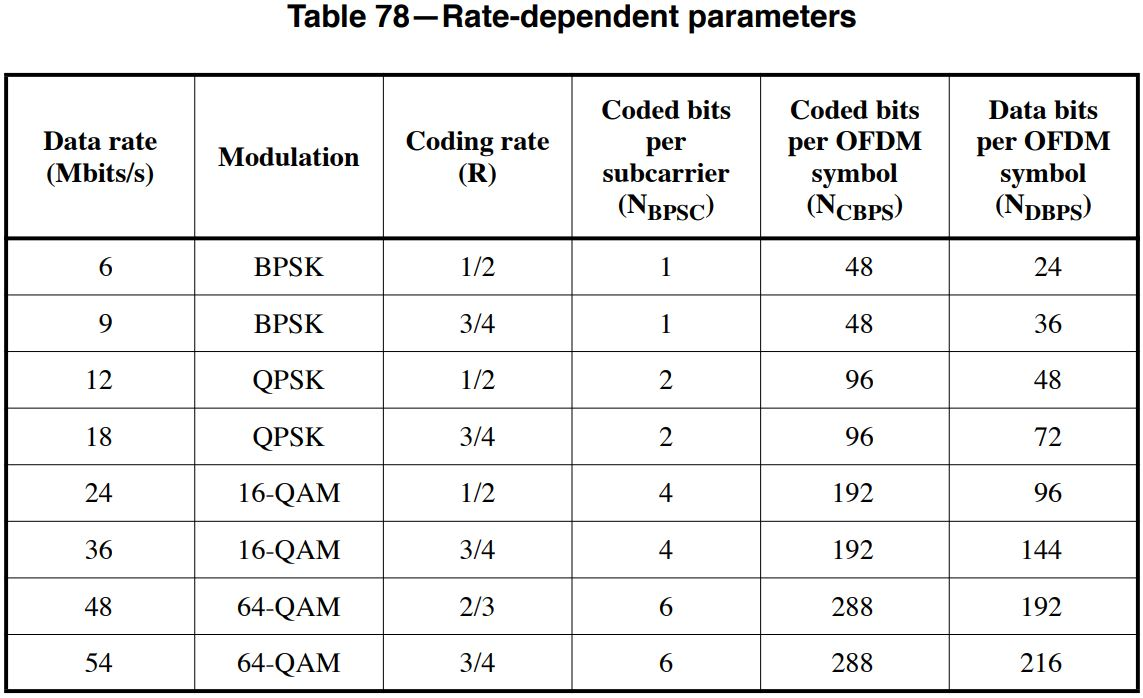
\includegraphics[width = 0.45\textwidth]{RateDepParams}
    \caption{Recreation of Table 78 --- Rate-Dependent Parameters}
    \label{fig:rate_params}
\end{figure}

In all eight modes of operation, timing parameters remain constant. These are represented in Fig~\ref{fig:time_params}.
\begin{figure}
    \centering
    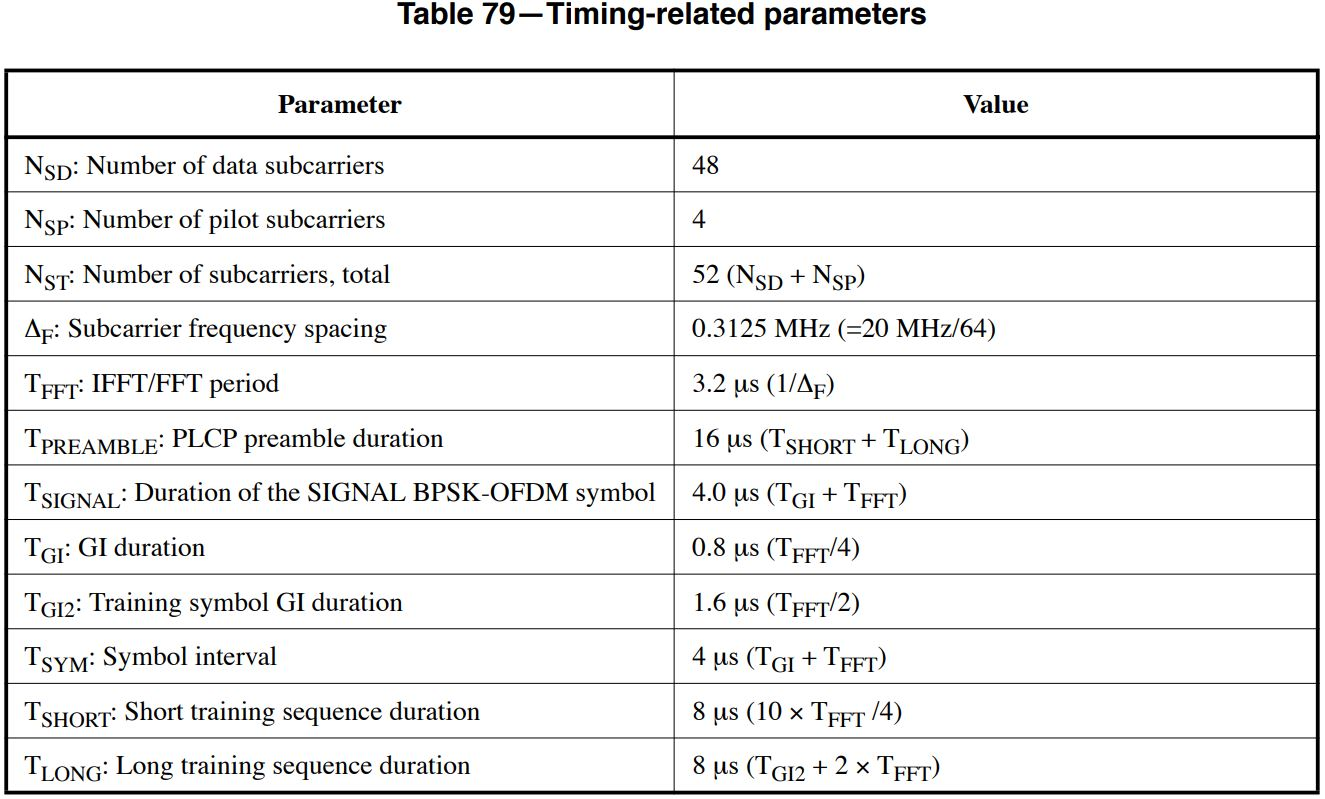
\includegraphics[width = 0.45\textwidth]{TimeDepParams}
    \caption{Recreation of Table 79 --- Timing-Related Parameters}
    \label{fig:time_params}
\end{figure}

Channels in the 5 GHz band are defined by their center frequencies, using the relation
\begin{equation}
\text{f}_\text{c} = 500 + 5 \times \text{n}_\text{ch},
\end{equation}
where $\text{n}_\text{ch} = 0,1,...,200$. However, due to regulation, not all channels are available for use; for the purpose of this project channel 36 was used in determining the center frequency.

\subsection{OFDM} \label{sec:OFDM}
OFDM, or \emph{Orthogonal Frequency-Division Multiplexing}, is a modulation scheme by which digital data is encoded onto multiple carrier frequencies within a certain frequency band, all spaced $\Delta_\text{F} = 1/\text{T}_\text{FFT}$ MHz apart. There is an additional condition that all subcarrier signals must be orthogonal to each other on the channel, thereby all but eliminating inter-carrier interference (ICI) and removing the need to include inter-carrier guard bands in the frequency domain (consequently allowing for a high spectral efficiency). An example of an OFDM spectrum across five subcarriers is presented in Fig~\ref{fig:OFDM}.
\begin{figure}
    \centering
    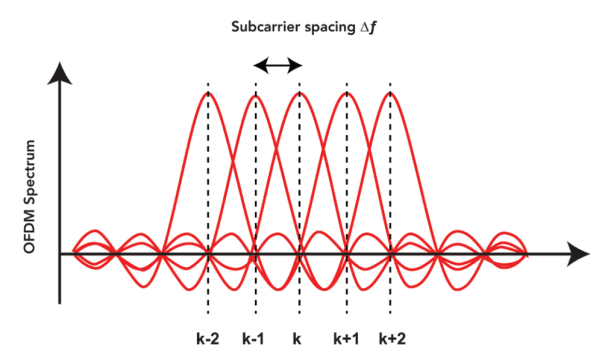
\includegraphics[width = 0.45\textwidth]{OFDM}
    \caption{Illustration of OFDM spectrum.}
    \label{fig:OFDM}
\end{figure}

This orthogonality principle lends to simple hardware translation as, fundamentally, one can use an inverse-forward pair of Fast Fourier Transform (FFT) blocks to facilitate this modulation on the transmitter and receiver, respectively. The 802.11 standard encodes forty-eight symbols at a time; combined with four pilot subcarriers, the frame is passed through a zero-padded IFFT (as shown in Fig.~\ref{fig:IFFT}).
\begin{figure}
    \centering
    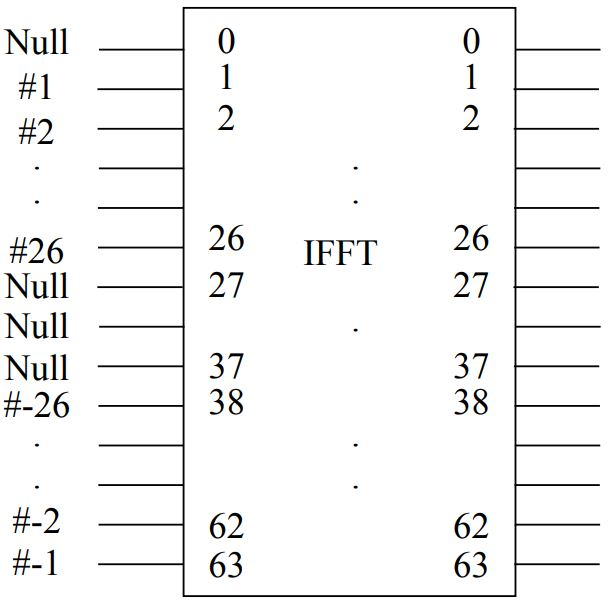
\includegraphics[width = 0.45\textwidth]{IFFT}
    \caption{Block diagram of symbol ordering on input to IFFT on the transmitter.}
    \label{fig:IFFT}
\end{figure}

Once in the time-domain, a cyclic prefix is prepended to the frame, consisting of the last sixteen time-domain samples out of the outputted sixty-four. This is easily apparent as, per Fig.~\ref{fig:time_params}, the required guard time $\text{T}_\text{GI}$ (which determines the time-frame that the cyclic prefix occupies) is a quarter of the IFFT/FFT period $\text{T}_\text{FFT}$. Therefore, the entire transmitted frame consists of a total of eighty time-domain samples (see Fig.~\ref{fig:Frame}).
\begin{figure}
    \centering
    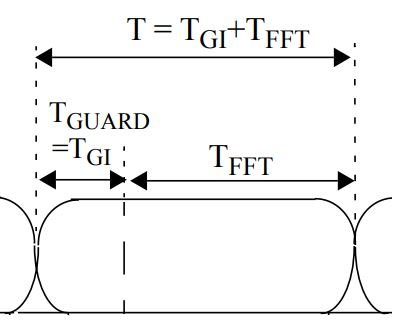
\includegraphics[width = 0.45\textwidth]{Frame}
    \caption{A single time-domain transmission frame, with guard time $\text{T}_\text{GI}$ and useful symbol time $\text{T}_\text{FFT}$ labeled.}
    \label{fig:Frame}
\end{figure}

At this stage, the signal is heterodyned for RF transmission across the channel, where it is received by the receiver, heterodyned back down to baseband, and OFDM demodulation takes place.

%%%%%%%%%%%%%%%%%%% Sections %%%%%%%%%%%%%%%%%%%
%\section{•} \label{sec:•}
%•

%%%%%%%%%%%%%%%%% Citation %%%%%%%%%%%%%%%%%%%%%%
%~\cite{•}

%%%%%%%%%%% Figures %%%%%%%%%%%%%%%%%%%%%
%\begin{figure}
%    \centering
%    \includegraphics[width = 0.45\textwidth]{•}
%    \caption{•}
%    \label{fig:•}
%\end{figure}

%%%%%%%%%%% Equation Array %%%%%%%%%%%%%%%%%%%%%
%\begin{eqnarray}
%• \nonumber \label{eq:•} \\
%& & • \label{eq:•}
%\end{eqnarray}

%%%%%%%%%%% Footnote %%%%%%%%%%%%%%%%%%%%%
%\footnote{• \label{fn:•}}

%%%%%%%%%%%%%%%%%%% Bibliography %%%%%%%%%%%%%%%%%%%
%\bibliographystyle{unsrt}	
%% To reload citations:
%% F6 --> F11 --> F6 --> F6 --> F7
%\bibliography{•} %filename (no .bib)

\end{document}